\documentclass[final]{beamer}
\usepackage[utf8]{inputenc}
\usepackage[english]{babel}
\usepackage[orientation=portrait,size=a0,scale=1.7]{beamerposter}
\usepackage{blindtext}

\usepackage{xcolor}
\usepackage{mdframed}

\usepackage{caption}
\captionsetup[figure]{labelformat=empty}

\geometry{
  hmargin=5cm,
}

\linespread{1.15}

\usetheme{sharelatex}

\title
[Conference name, 1 - 5 March, Location]
{Poster title - \newline Poster subtitle}

\author{ % Authors
First Last\inst{1} \url{mail@domain.org}
}
\institute
[Freie Universität Berlin]
{
\inst{1} Biorobotics Lab Berlin \url{biorobotics.mi.fu-berlin.de}\\[0.3ex]
}
\date{\today}

\begin{document}
\begin{frame}[t]
\begin{multicols}{3}

\justifying

\begin{figure}
    \begin{mdframed}[backgroundcolor=black!2,userdefinedwidth=\columnwidth,linewidth=0pt]
    \centering
    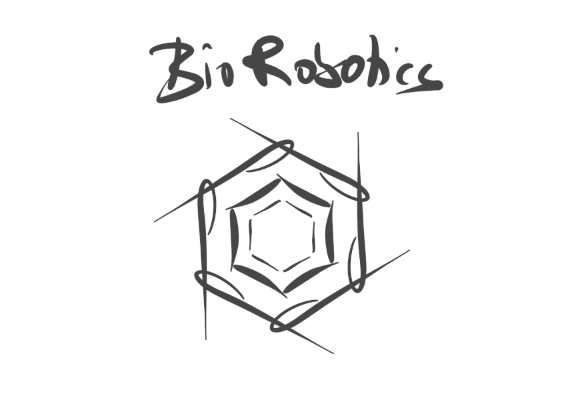
\includegraphics[width=0.96\columnwidth]{image/biorobotics}
    \caption{\small Figure caption}
    \label{fig:lab_logo}
    \end{mdframed}
\end{figure}

\blindtext[1]

$
f_{i, t}=m_\theta (a_i^t) + o(i, a_i^t) \\
o_{i, t}=h_\phi (e_\omega(i), a_i^t) \\
p_{i, j, t} \approx f_{i, t} \cdot f_{j, t}^T \approx m_\theta (a_i^t) \cdot m_\theta (a_j^t)^T
$

\blindtext[2]

\begin{figure}
    \begin{mdframed}[backgroundcolor=black!2,userdefinedwidth=\columnwidth,linewidth=0pt]
    \centering
    
\includegraphics[width=0.96\columnwidth]{image/fuberlin}
    \caption{\small Figure caption}
    \label{fig:lab_logo}
    \end{mdframed}
\end{figure}

\blindtext[1]

$
f_{i, t}=m_\theta (a_i^t) + o(i, a_i^t) \\
o_{i, t}=h_\phi (e_\omega(i), a_i^t) \\
p_{i, j, t} \approx f_{i, t} \cdot f_{j, t}^T \approx m_\theta (a_i^t) \cdot m_\theta (a_j^t)^T
$

\blindtext[2]

\end{multicols}
\end{frame}
\end{document}